\chapter{Diseño e Implementación} % Main chapter title

\label{Chapter3} % Change X to a consecutive number; for referencing this chapter elsewhere, use \ref{ChapterX}
\definecolor{mygreen}{rgb}{0,0.6,0}
\definecolor{mygray}{rgb}{0.5,0.5,0.5}
\definecolor{mymauve}{rgb}{0.58,0,0.82}

\lstset{ %
  backgroundcolor=\color{white},   % choose the background color; you must add \usepackage{color} or \usepackage{xcolor}
  basicstyle=\footnotesize,        % the size of the fonts that are used for the code
  breakatwhitespace=false,         % sets if automatic breaks should only happen at whitespace
  breaklines=true,                 % sets automatic line breaking
  captionpos=b,                    % sets the caption-position to bottom
  commentstyle=\color{mygray},    % comment style
  deletekeywords={...},            % if you want to delete keywords from the given language
  %escapeinside={\%*}{*)},          % if you want to add LaTeX within your code
  %extendedchars=true,              % lets you use non-ASCII characters; for 8-bits encodings only, does not work with UTF-8
  %frame=single,	                   % adds a frame around the code
  keepspaces=true,                 % keeps spaces in text, useful for keeping indentation of code (possibly needs columns=flexible)
  keywordstyle=\bfseries\color{black},       % keyword style
  language=[ANSI]C,					% the language of the code
  %otherkeywords={*,...},           % if you want to add more keywords to the set
  numbers=left,                    % where to put the line-numbers; possible values are (none, left, right)
  numbersep=5pt,                   % how far the line-numbers are from the code
  numberstyle=\tiny\color{mygray}, % the style that is used for the line-numbers
  rulecolor=\color{black},         % if not set, the frame-color may be changed on line-breaks within not-black text (e.g. comments (green here))
  showspaces=false,                % show spaces everywhere adding particular underscores; it overrides 'showstringspaces'
  showstringspaces=false,          % underline spaces within strings only
  showtabs=false,                  % show tabs within strings adding particular underscores
  stepnumber=1,                    % the step between two line-numbers. If it's 1, each line will be numbered
  stringstyle=\bfseries\color{black},     % string literal style
  tabsize=2,	                   % sets default tabsize to 2 spaces
  title=\lstname,                   % show the filename of files included with \lstinputlisting; also try caption instead of title
  morecomment=[s]{/*}{*/}%
}


En este capítulo se detalla el desarrollo del firmware, software y documentación.

%----------------------------------------------------------------------------------------
%	SECTION 1 : Diseño de Firmware
%----------------------------------------------------------------------------------------
\section{Diseño del Firmware}

\subsection{Punto de partida} 

Al tomar el port de MicroPython para la EDU-CIAA-NXP desarrollado por Martín Ribelotta, era posible ejecutar un intérprete \textit{REPL}\footnote{REPL: Read Eval Print Loop. Mecanismo que toma una expresión escrita por el usuario, la evalúa y ejecuta, devolviendo el resultado al usuario.} que provee el proyecto, el cual tiene como standard input (stdin) y standard output (stdout) el puerto serie que la placa tiene conectado a través del conversor USB, de modo que en la PC se crea un COM Virtual que permite a cualquier programa que emula una terminal por puerto serial, conectarse a dicho intérprete.

En la figura \ref{fig:conexion} se observan los bloques que modelan la conexión de la placa con la PC. Mediante el circuito integrado FT2232 que posee la placa, se conecta por medio del bus USB, la PC a la EDU-CIAA-NXP, permitiendo visualizar uno de los módulos UART del microcontrolador como un puerto serie en la PC.

\begin{figure}[h]
  \centering
    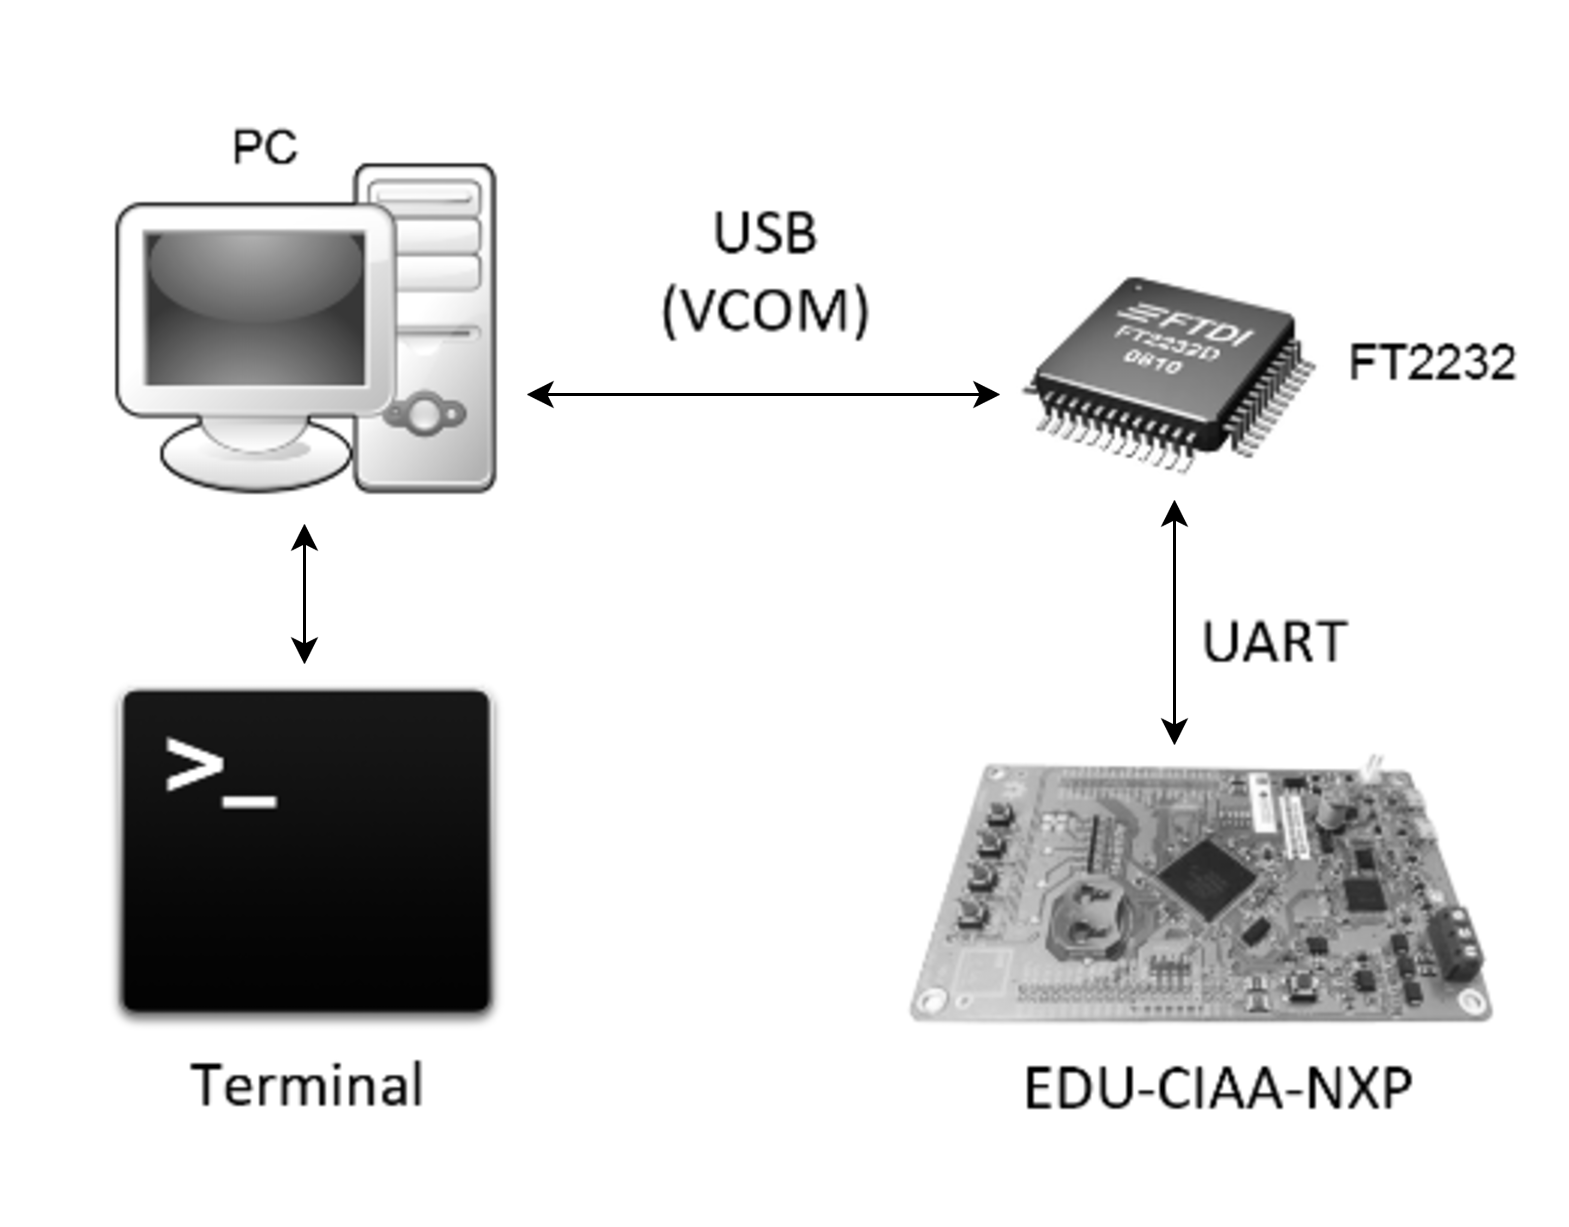
\includegraphics[width=0.7\textwidth]{Figures/fig_conexion}
  \caption{Conexión de la EDU-CIAA-NXP con la PC}
  \label{fig:conexion}
\end{figure}

Esto permite ejecutar programas que no tengan interacción con el resto del hardware, por ejemplo, se puede escribir:

\textbf{{\fontsize{16}{16}\selectfont \textgreater\textgreater}} \texttt{print(“Hola mundo”)}

Una vez ingresado el código, el interprete lo evalúa y ejecuta, y el texto "Hola mundo" se transmite por el stdout, el cual está ligado a la UART conectada al conversor serie-USB, por lo que el texto "Hola mundo" se muestra por la terminal de la PC.

De la misma forma se puede utilizar el sdtin con sentencias como:

\textbf{{\fontsize{16}{16}\selectfont \textgreater\textgreater}} \texttt{n = input(“Ingrese un numero”)}

También se pueden realizar operaciones matemáticas como por ejemplo:

\textbf{{\fontsize{16}{16}\selectfont \textgreater\textgreater}} \texttt{a = 27}\\
\textbf{{\fontsize{16}{16}\selectfont \textgreater\textgreater}} \texttt{b = 3}\\
\textbf{{\fontsize{16}{16}\selectfont \textgreater\textgreater}} \texttt{c = a + b}\\
\textbf{{\fontsize{16}{16}\selectfont \textgreater\textgreater}} \texttt{print(c)}

Este último ejemplo imprime por la terminal el valor 30.

Pero para interactuar con los periféricos como los pulsadores y los leds, solo existía una versión preliminar de algunas bibliotecas Python creadas previamente por el autor de este trabajo, las cuales se tomaron como punto de partida para el desarrollo profesional de las mismas verificando su correcto funcionamiento por medio de test unitarios y funcionales los cuales son explicados en el capítulo \ref{Chapter4}.

%----------------------------------------------------------------------------------------

\subsection{Creación de bibliotecas Python: Módulos y Clases} 

Si bien es posible definir funciones sueltas sin contexto, en Python también es posible la declaración de clases, al ser un lenguaje multiparadigma, el mismo contempla la Programación Orientada a Objetos (POO), mediante la cual se modelaron los periféricos del microcontrolador.

En Python, las clases se agrupan dentro de módulos. Un módulo Python es un conjunto de clases, para poder utilizar una clase que se encuentra dentro de un módulo, deberemos incluir dicho módulo en nuestro programa, mediante la sentencia import, por ejemplo:

\textbf{{\fontsize{16}{16}\selectfont \textgreater\textgreater}} \texttt{import pyb}

El módulo pyb tiene dentro definidas las clases que representan los periféricos del microcontrolador. Una vez incluído el módulo, podremos utilizar las clases definidas dentro de él para crear objetos.
Por ejemplo, para la creación de un objeto que representa el led 1 de la EDU-CIAA-NXP, se escribe:

\textbf{{\fontsize{16}{16}\selectfont \textgreater\textgreater}} \texttt{import pyb}\\
\textbf{{\fontsize{16}{16}\selectfont \textgreater\textgreater}} \texttt{led = pyb.LED(1)}\\
\textbf{{\fontsize{16}{16}\selectfont \textgreater\textgreater}} \texttt{led.on()}

En este ejemplo se utiliza la clase LED para crear el objeto led, la misma recibe como argumento de su constructor, el número de led que el objeto manejará, en este caso, el led 1.

Para poder manejar un periférico del microcontrolador (GPIOs, UART, etc.) es necesario que al ejecutar una o más funciones de código Python, se ejecute una o más funciones de código C, en la cual se coloca el código necesario para la utilización del periférico en cuestión.

En la figura \ref{fig:calls} se muestra un diagrama donde se aprecia el \textit{trace}\footnote{Tracing: Log que muestra información acerca de la ejecución de un programa junto con las llamadas a funciones.} de las llamadas a función que se ejecutan cuando el usuario ejecuta desde código Python el método on() de un objeto LED.

\begin{figure}[ht]
  \centering
    \includegraphics[width=1.05\textwidth]{Figures/fig_calls}
  \caption{Anidamiento de llamadas a funciones desde Python a C}
  \label{fig:calls}
\end{figure}

Al ejecutarse la llamada del método on() desde el objeto led, se produce la ejecución de la función pyb\_led\_on() la cual se encuentra definida en el archivo modpybled.c, en este archivo están declaradas todas las funciones que se mapean a métodos del objeto LED. Cada método que pose el objeto led tendrá asociada una función dentro del archivo modpybled.c.

Estos archivos modpybXXX.c representan la clase de un periférico (en este ejemplo modpybled.c representa la clase LED) y utilizan las funciones de la capa de abstracción de hardware (uPython HAL) definidas en ciaanxp\_mphal.c para acceder y utilizar los periféricos.
Dentro de la capa uPython HAL, se utilizan las funciones definidas en la capa Board Support Package (archivo board.c) en donde se utilizan las funciones de la biblioteca \textit{LPCOpen}\footnote{LPCOpen: Biblioteca desarrollada por NXP la cual provee macros y funciones para acceder a los registros del microcontrolador desde lenguaje C.} para el manejo de periféricos.

En la figura \ref{fig:files} se observan los archivos implicados para poder brindar desde el código Python una interfaz para el uso de cada periférico. En ella se observa que existe un archivo modpybXXX.c para definir cada clase Python. Dentro de cada archivo se definen las funciones de C que se ejecutarán al invocar los métodos desde Python. Estas funciones de C utilizan la capa uPython HAL para interactuar con los periféricos del microcontrolador.
Para una explicación detallada sobre el desarrollo de una clase Python desde código C, referirse al apéndice \ref{AppendixA}

\begin{figure}[ht]
  \centering
    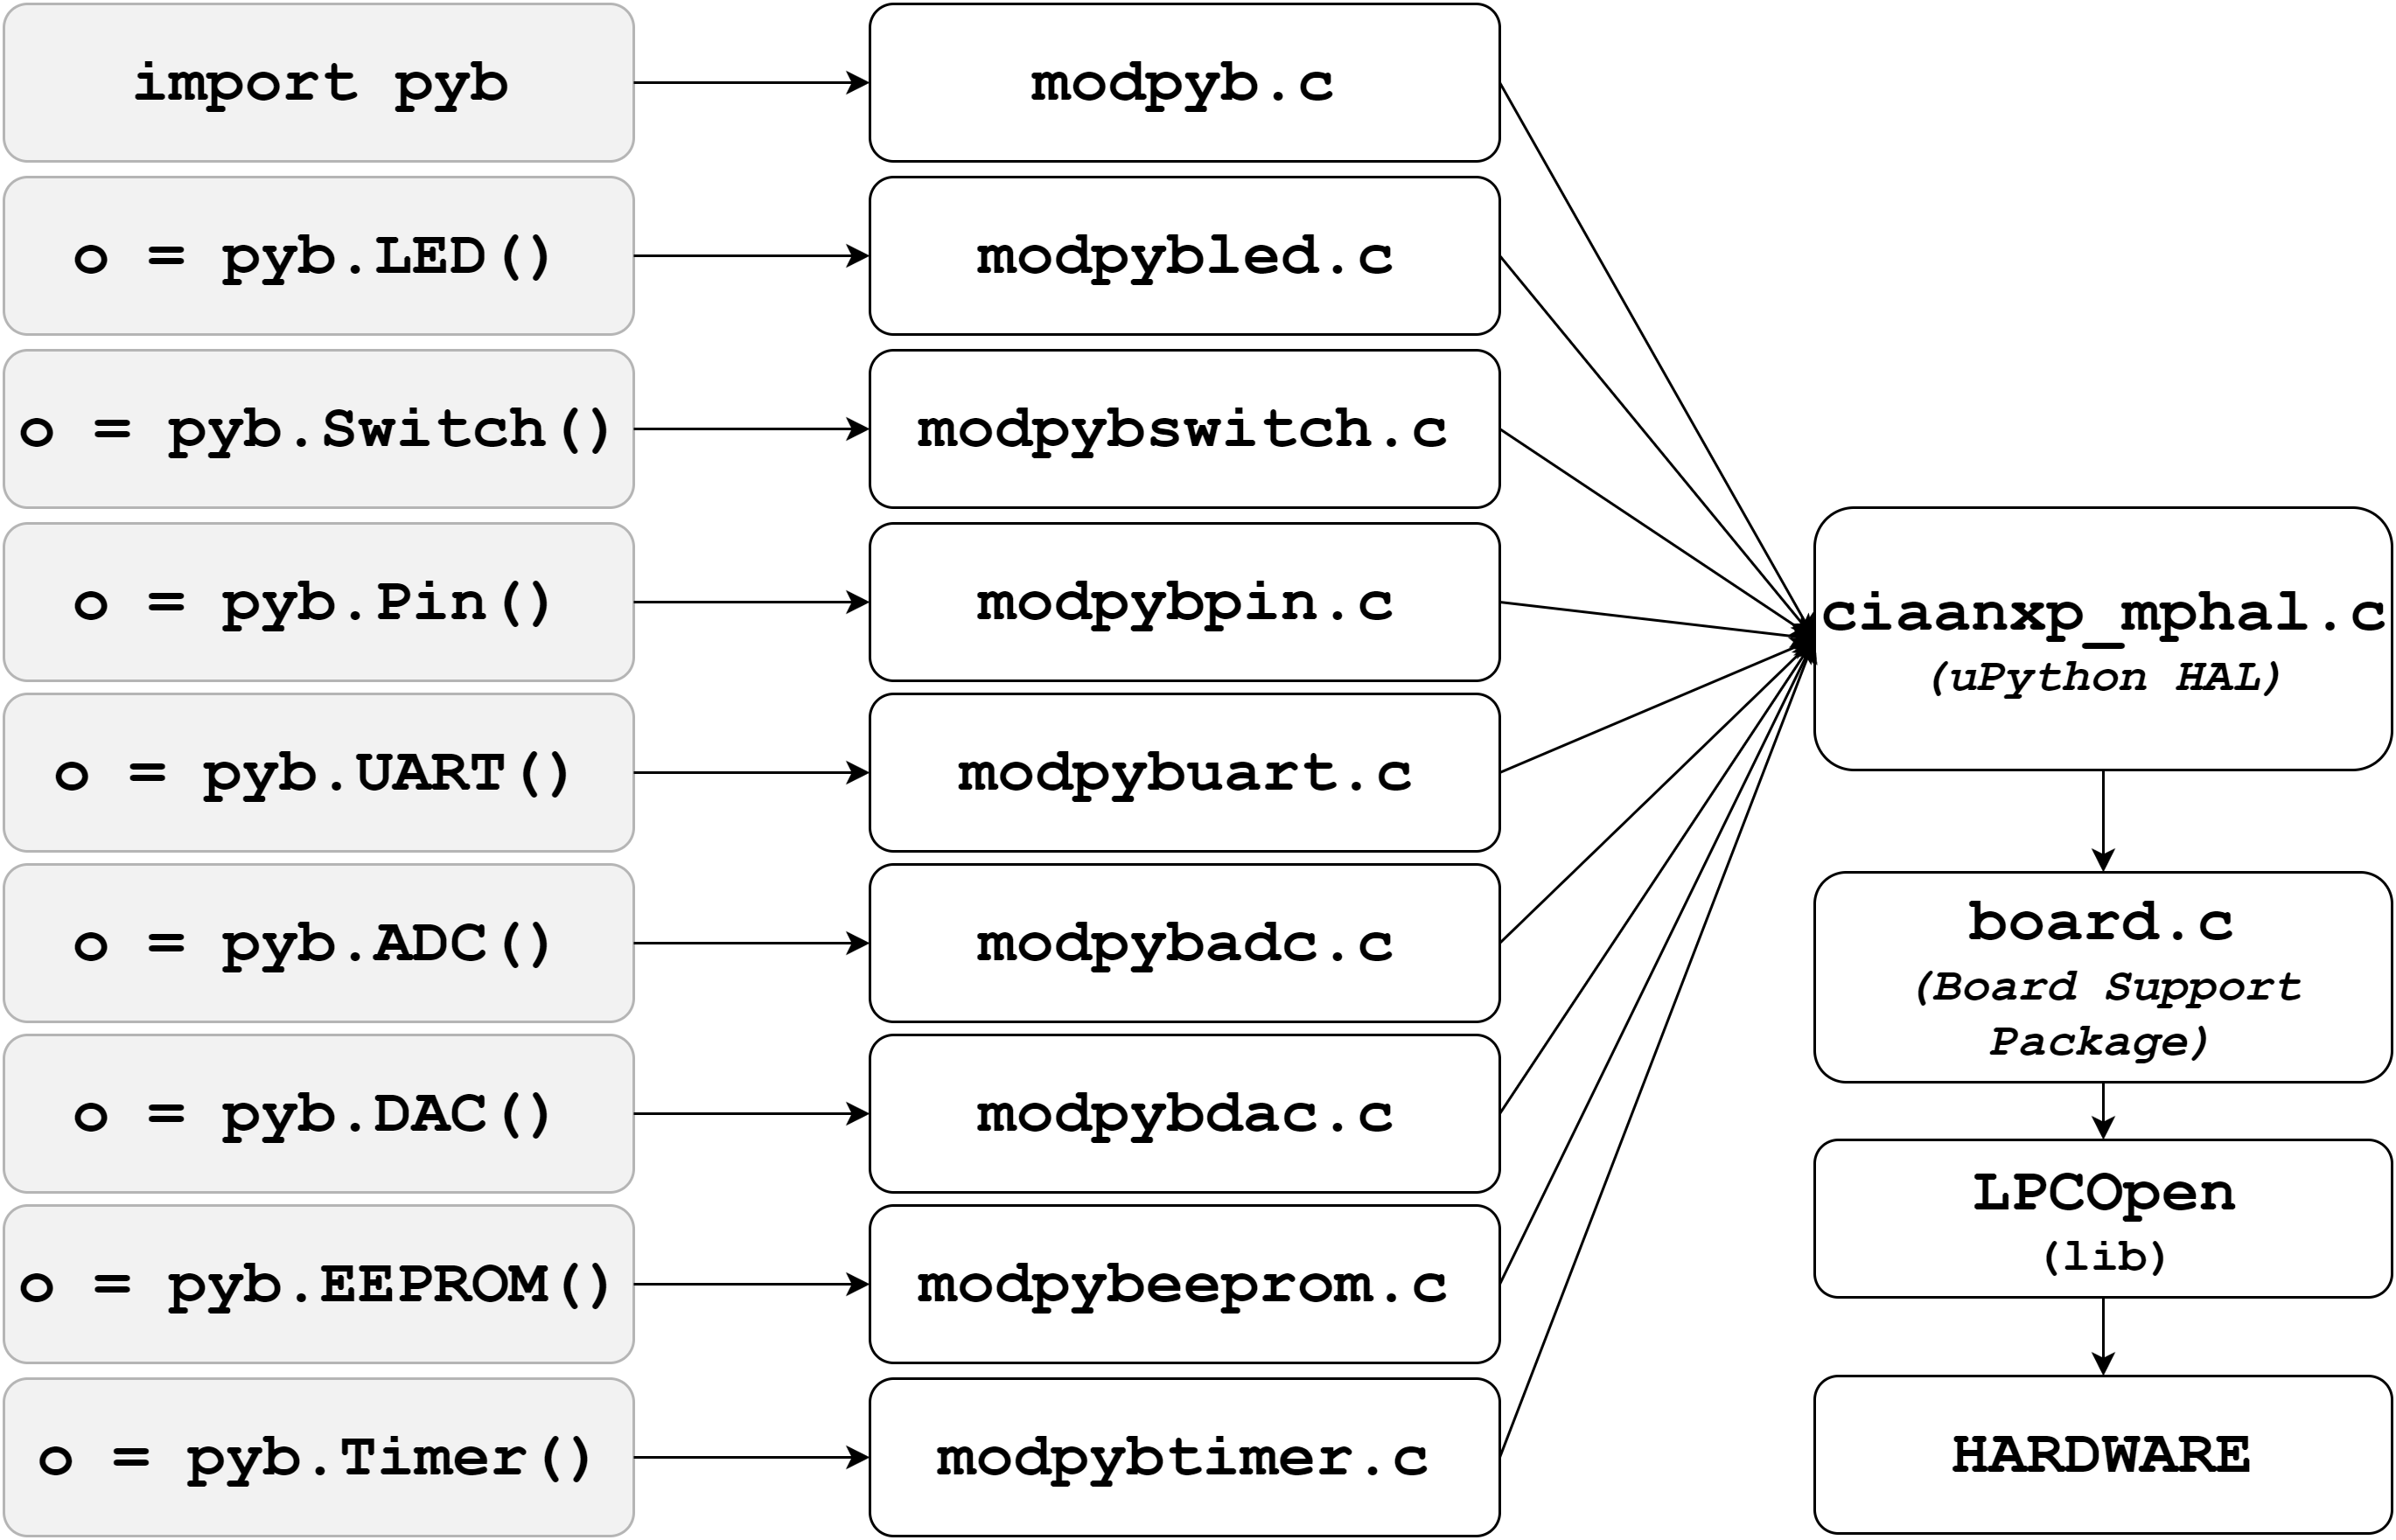
\includegraphics[width=0.95\textwidth]{Figures/fig_files}
  \caption{Relación entre las clases Python y los archivos del firmware}
  \label{fig:files}
\end{figure}

%----------------------------------------------------------------------------------------

\subsection{Diseño de bibliotecas para el manejo de periféricos desde C}

En el archivo board.c y board.h se definió la capa Board Support Package (BSP), mediante la cual se accede a los periféricos del microcontrolador, en este archivo se definieron las funciones para inicializar y utilizar dichos periféricos, requiriendo la menor cantidad de datos de inicialización posibles y abstrayendo en gran medida la arquitectura del microprocesador.

Esta capa utiliza la biblioteca LPCOpen, la cual es de más bajo nivel pero permite un fácil acceso a los registros del microcontrolador, proveyendo funciones y macros para resolver este problema.

Las funciones definidas en board.c tienen el formato:

\begin{verbatim}
Board_NombrePeriferico_NombreFuncion()
\end{verbatim}

Algunos ejemplos de las funciones que pueden encontrarse en este archivo son:

\begin{verbatim}
void Board_LED_Set(uint8_t LEDNumber, bool On);
bool Board_LED_Test(uint8_t LEDNumber);
void Board_LED_Toggle(uint8_t LEDNumber);
\end{verbatim}

Todos los periféricos tienen su función Init:
\begin{verbatim}
Board_NombrePeriferico_Init()
\end{verbatim}

la cual se encarga de inicializar dicho periférico. Existe también en el archivo, definida una función principal que se encarga de llamar a todas las funciones “Init” y es llamada “Board\_Init()”

Como se indica en la figura \ref{fig:calls}, las funciones definidas en esta capa son ejecutadas por las funciones definidas en la capa uPython HAL, las cuales se definen en el archivo ciaanxp\_mphal.c y ciaanxp\_mphal.h.

La capa uPython HAL, es prácticamente transparente, ya que en la mayoría de los casos no agrega funcionalidades, y simplemente invoca a las funciones de la capa BSP. 
Sin embargo en algunos casos en donde las funciones definidas en BSP no cubren las características necesarias para ser utilizadas desde Python, se han agregado las características en esta capa.

También se han agregado porciones de código para validación de rangos o para agregar argumentos, como se muestra en el algoritmo \ref{lst:uarthal} en donde se define la función para enviar por el puerto serie.

\begin{lstlisting}[label={lst:uarthal},caption=Función de envío por la UART de la capa uPython HAL] 
uint32_t mp_hal_rs232_write(uint8_t const * const buffer, 
                                     uint32_t size,uint32_t delay)
{
    if(delay==0)
        return Board_UART_Write(LPC_USART3,buffer,size);

    uint32_t i=0;
    while(size>0)
    {
        Board_UART_Write(LPC_USART3,&(buffer[i]),1);
        mp_hal_milli_delay(delay);
        size--;
        i++;
    }
    return i;
}
\end{lstlisting}

En este caso se observa que la función de la capa uPython HAL tiene un argumento que indica un retardo (delay) entre cada byte que se envía (línea 2), funcionalidad que no existe en la capa BSP, ya que solo se dispone de la función “Board\_UART\_Write()” la cual recibe el buffer a transmitir.
En esta función se evalúa el valor del argumento delay, y en el caso de que sea mayor a cero, se harán envíos de 1 byte y por cada envío se ejecutará la función “mp\_hal\_milli\_delay()” la cual boquea el código por el tiempo especificado.

Las funciones de la capa uPython HAL tienen la forma:

\begin{verbatim}
mp_hal_nombrePeriferico_nombreFuncion()
\end{verbatim}

Tanto la biblioteca BSP como la capa uPython HAL pueden utilizarse de forma aislada en un proyecto \textit{baremetal}\footnote{Baremetal: Método de programación de bajo nivel para un hardware específico utilizando herramientas básicas y sin un sistema operativo.} para el microcontrolador LPC4337, proveyendo un acceso simple a los periféricos del mismo.

%----------------------------------------------------------------------------------------

\subsection{Diseño de bibliotecas para el manejo de periféricos desde el código Python}

Se pretendió modelar cada periférico mediante una clase, si bien era posible definir funciones pertenecientes al módulo pyb, sin definir clases, por ejemplo:

\textbf{{\fontsize{16}{16}\selectfont \textgreater\textgreater}} \texttt{pyb.setLed(1,0)}

Se decidió respetar el modelo orientado a objetos por las siguientes razones:

\begin{itemize}
	\item El proyecto MicroPython original utiliza este modelo para acceder a los periféricos.
	\item Ayuda al entendimiento de programación orientada a objetos (POO), en donde la premisa más básica es representar objetos del mundo real, en este caso un objeto Switch representará un pulsador físico en la placa, generando un ejemplo muy claro del concepto.
	\item Para el uso básico y explicaciones de algoritmo, no es necesario tener los conocimientos de POO, simplemente se trata al objeto como una variable, y no se generan grandes trabas en el momento del aprendizaje.
\end{itemize}

En la figura \ref{fig:classes} se observa el diagrama de clases definido para el módulo pyb, en donde se encuentran las clases que representan los periféricos del microcontrolador junto con los métodos desarrollados.

\begin{figure}[ht]
  \centering
    \includegraphics[width=1.1\textwidth]{Figures/fig_classes_diagram}
  \caption{Diagrama de clases para manejo de periféricos}
  \label{fig:classes}
\end{figure}

%----------------------------------------------------------------------------------------
%	SECTION 2: Diseño del Software
%----------------------------------------------------------------------------------------
\section{Diseño del Software}

\subsection{Punto de partida} 

Para el desarrollo del IDE se tomó como base el proyecto EDILE \cite{edile} el cual se muestra en la figura \ref{fig:edile}. El mismo se encuentra escrito en lenguaje Python y proporciona un procesador de texto con coloreado de palabras clave según el lenguaje seleccionado, el cual se detecta automáticamente por la extensión del archivo que se abre.

\begin{figure}[ht]
  \centering
    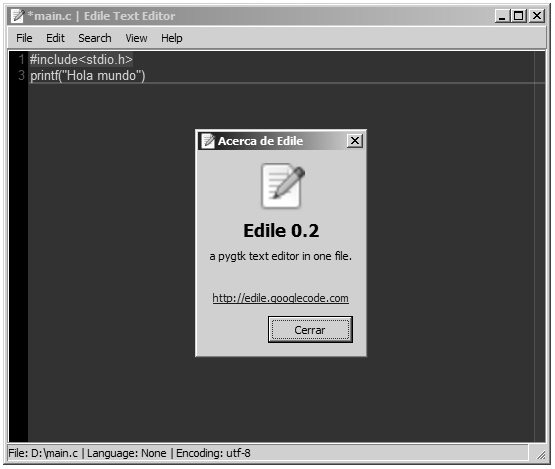
\includegraphics[width=0.7\textwidth]{Figures/fig_edile}
  \caption{Procesador de texto EDILE v0.2}
  \label{fig:edile}
\end{figure}

Debido a que se encuentra programado en Python es muy simple ejecutar el programa en diferentes sistemas operativos, de modo que utilizando este proyecto se puede cumplir con uno de los requerimientos planteados el cual decía que el software debe ser multiplataforma.

Este procesador de texto posee un sistema de plug-ins mediante el cual se simplifica la incorporación de menúes que ejecuten ventanas adicionales que cumplan con cierta funcionalidad, de modo que el diseño de software que se realizó en el presente trabajo fue la incorporación de dichas ventanas y funcionalidades al editor, junto con modificaciones para que solo trabaje con archivos de código Python (.py) y algunas correcciones en el sistema de plug-ins.

Junto con las modificaciones mencionadas, se escribieron test unitarios para las ventanas y clases de lógica desarrolladas, asegurando al igual que en el firmware, la calidad del software requerida para un trabajo de especialización.

\subsection{Diseño del IDE} 

Se modificó el código del proyecto EDILE y se incorporó una barra de botones junto con una nueva opción de menú, llamada “EDU-CIAA”. La incorporación de este nuevo menú fue posible gracias al sistema de plug-ins con el que cuenta en editor base, en la figura \ref{fig:idebuttons} se aprecia el menú agregado así como también los botones que poseen las mismas funcionalidades que las opciones del menú.

\begin{figure}[ht]
  \centering
    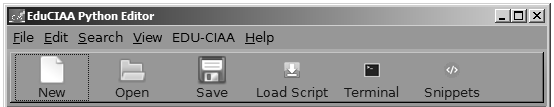
\includegraphics[width=0.7\textwidth]{Figures/fig_ide_buttons}
  \caption{Botones adicionales del IDE.}
  \label{fig:idebuttons}
\end{figure}

En la figura \ref{fig:ideclasses} se observan las clases desarrolladas. La clase que funciona como un plug-in del editor, es la llamada mnu\_EDUCIAA, en ella se ejecutan métodos según qué opción de menú eligió el usuario (o que botón presionó). Esta clase hace las veces de \textit{controller}\footnote{controller: Componente del patrón de diseño MVC el cual se encarga de recibir eventos y realizar acciones.} y dispara las diferentes ventanas según la opción seleccionada.

\begin{figure}[ht]
  \centering
    \includegraphics[width=0.99\textwidth]{Figures/fig_ide_classes}
  \caption{Diagrama de clases de las funcionalidades agregadas al IDE.}
  \label{fig:ideclasses}
\end{figure}

 A continuación se detallan las clases creadas:

\begin{itemize}
	\item \textbf{mnu\_EDUCIAA}: recibe los eventos de click sobre los ítems del menú o los botones y lanza las diferentes ventanas (Terminal serie, Configuración, Snippets y Grabación).
	\item \textbf{Console}: ventana que se conecta por el puerto serial configurado y muestra en pantalla los caracteres recibidos, de la misma forma captura las teclas que el usuario presiona y las envía.
	\item \textbf{ConfigWindow}: ventana que permite al usuario configurar el puerto serie mediante el cual se comunica el IDE con la EDU-CIAA-NXP.
	\item \textbf{SnippetsWindow}: ventana que muestra una lista de porciones de código de ejemplo, y que por medio de un botón permite agregarlas al texto que el usuario está escribiendo.
	\item \textbf{LoadScriptWindow}: ventana que se encarga del envío del archivo a la placa utilizando el protocolo xmodem y de mostrar el progreso.
	\item \textbf{ConfigManager}: esta clase se encarga de escribir y leer en un archivo la configuración del IDE (es decir el puerto serie que seleccionó el usuario).
	\item \textbf{SnippetsParser}: todos los ejemplos que se muestran en la ventana de Snippets, se leen de un archivo XML. Esta clase se encarga de leer dicho archivo y devolver la información para que la ventana la pueda mostrar.	
	\item \textbf{Protocol}: recibe como dato el puerto serie y la ruta al archivo a transmitir, y se encarga de utilizar la biblioteca XMODEM para enviar el archivo hacia la placa.
	\item \textbf{XMODEM}: biblioteca que implementa el protocolo \textit{xmodem}\footnote{xmodem: Protocolo simple de transferencia de datos por medio de paquetes de 128bytes creado en 1977.} y permite el envío del archivo a la placa.	
\end{itemize}

El diseño de las ventanas y sus contenidos fueron creados con el programa Glade\cite{glade} utilizado para crear ventanas para la biblioteca gráfica pyGTK.

La lógica de cada ventana se encuentra implementada dentro de cada una de las clases, las cuales utilizan la biblioteca pyGTK para construir la interfaz gráfica por medio de un archivo XML (extensión .glade) donde se define el formato de la ventana y los componentes que posee dentro (Botones, etc.)

En el algoritmo \ref{lst:pygtkbuilder} se muestra la creación del objeto builder el cual obtiene los datos de la ventana gráfica del archivo LoadScriptWindow.glade, archivo creado con el programa Glade. Luego en la línea 8 se observa cómo mediante el método get\_objet() se obtiene una referencia de un objeto Button definido para dicha ventana y que tiene asignado el nombre “btnClose”. De esta manera se obtienen las referencias de los objetos definidos en el archivo XML y que componen la ventana, permitiendo la interacción con los mismos desde el código.

\begin{lstlisting}[language={python},label={lst:pygtkbuilder},caption=Porción de código que muestra la creación de la ventana a partir del archivo glade] 
		try:
			builder = gtk.Builder()
			builder.add_from_file(basePath+"/LoadScriptWindow.glade")
		except Exception,e:
			print(e)
			return

		self.buttonClose = builder.get_object("btnClose")
		
\end{lstlisting}

\subsection{Envío del archivo a la placa}

Para el envío del archivo a la placa, se utilizó el protocolo xmodem debido a su sencillez, este protocolo permite la trasferencia de datos en paquetes de 128 bytes o 1kbytes, por cada paquete transferido el receptor envía un acuse de recibo (ACK) o un aviso de que hubo un error (NACK).

En la figura \ref{fig:secuencexmodem} se observa el diagrama de secuencia correspondiente a la transferencia de datos entre el firmware desarrollado y la lógica de la ventana LoadScriptWindow.
En él se observa que al reiniciar la placa mediante su pulsador de reset, el firmware envía una trama NACK por el puerto serie, en el caso de que el IDE se encuentre en el modo de inicializar una grabación (porque el usuario abrió la ventana de grabación) se recibirá dicha trama y se reponderá con el primer paquete de datos de 128bytes, al cual el firmware que recibe dicha trama responderá con ACK si pudo grabarlo en la memoria de programa del microcontrolador o NACK en caso de error. 

\begin{figure}[ht]
  \centering
    \includegraphics[width=0.6\textwidth]{Figures/fig_ide_xmodem}
  \caption{Diagrama de secuencia que describe la comunicación entre el IDE y el firmware.}
  \label{fig:secuencexmodem}
\end{figure}

Este proceso continúa hasta que el IDE envía todas las tramas que corresponden al contenido del archivo que se esta enviando.
El firmware irá agregando los datos recibidos al final de la memoria donde se grabaron los datos de la trama anterior.



%----------------------------------------------------------------------------------------
%	SECTION 3: Documentacion
%----------------------------------------------------------------------------------------
\section{Documentación}

Como se indica en el capítulo \ref{Chapter1}, el desarrollo del firmware y del software no es suficiente para que un proyecto educativo tenga el impacto deseado, sino que debe estar acompañado por la documentación y los ejemplos adecuados. Esta es la razón por la que el IDE posee una ventana de Snippets con porciones de código de ejemplo, sin embargo esto no es suficiente, ya que no existe explicación alguna de dichas porciones de código. 
Además de los Snippets, se agregaron proyectos de ejemplo y documentación de las clases y métodos desarrollados para el manejo de los periféricos.

\subsection{Proyectos de ejemplo} 

Para la publicación de ejemplos completos, se creó un repositorio público en GitHub\cite{repoejemplos} en donde pueden descargarse diferentes tipos de proyectos con una explicación detallada del código que se implementó. Los ejemplos se dividen en tres categorías:

\begin{itemize}
	\item \textbf{Inicial}: cubren conceptos básicos de programación y del lenguaje Python.
	\item \textbf{Intermedio}: proyectos que requieren conocimientos intermedios de programación y básicos de electrónica.
	\item \textbf{Avanzado}: proyectos que requieren conocimientos avanzados de programación y electrónica..	
\end{itemize}

Cada proyecto es acompañado por un archivo README.md en donde se aclaran las funciones y sentencias utilizadas, y se explica el funcionamiento del código paso por paso.

La idea es que la comunidad que utilice esta plataforma para desarrollar trabajos, en escuelas secundarias o universidades, aporte los trabajos implementados al repositorio, para que otros estudiantes puedan tomarlos como base para nuevos proyectos o simplemente para aprender de lo desarrollado.

\subsection{Documentación de las bibliotecas implementadas} 

Para acompañar a los proyectos de ejemplo y dar una base sólida del uso y soporte de los periféricos, se escribió una documentación detallada de cada clase con todos sus métodos, escribiendo también uno o más ejemplos del uso de algunos métodos en particular.

Esta documentación se escribió en la página del proyecto CIAA, en la sección Python\cite{bibpython}, la cual también es de acceso público, cumpliendo así con uno de los requerimientos mencionados en el capítulo \ref{Chapter2}. El link a esta página se encuentra accesible desde la ventana de Snippets del IDE.







